\documentclass[11pt]{article}
\usepackage[T1]{fontenc}
\usepackage{lmodern}
\usepackage{microtype}
\usepackage[a4paper,margin=2.5cm]{geometry}
\usepackage{amsmath,amssymb,amsthm,mathtools}
\usepackage{graphicx,booktabs,array,enumitem,multirow}
\usepackage{xcolor}
\usepackage[hidelinks]{hyperref}
\usepackage[labelfont=bf]{caption}
\usepackage{tikz}
\usetikzlibrary{arrows.meta,positioning,fit,backgrounds}
\usepackage{pgfplots}
\pgfplotsset{compat=1.18}
\usepgfplotslibrary{groupplots}
\usepackage[most]{tcolorbox}

\newtheorem{theorem}{Theorem}
\newtheorem{proposition}{Proposition}
\newtheorem{lemma}{Lemma}
\newtheorem{corollary}{Corollary}
\theoremstyle{definition}
\newtheorem{definition}{Definition}
\newtheorem{remark}{Remark}

\newcommand{\X}{\mathcal{X}}
\newcommand{\Del}{\Delta(\X)}
\newcommand{\E}{\mathbb{E}}
\newcommand{\R}{\mathbb{R}}
\newcommand{\one}{\mathbf{1}}
\newcommand{\KL}{\mathrm{KL}}
\newcommand{\Mcomp}{\mathcal{M}_{\mathrm{comp}}}

\definecolor{ntp}{HTML}{2F6DB5}
\definecolor{brier}{HTML}{D9822B}
\definecolor{pg}{HTML}{3E9651}
\definecolor{pgb}{HTML}{8E5BB3}
\definecolor{boxbg}{HTML}{F3F6FA}

\newtcolorbox{thesis}[1][]{colback=boxbg,colframe=ntp!70!black,boxrule=0.6pt,arc=2pt,
  left=6pt,right=6pt,top=4pt,bottom=4pt,fonttitle=\bfseries,title=#1}
\newtcolorbox{plain}[1][]{colback=white,colframe=black!35,boxrule=0.5pt,arc=2pt,
  left=6pt,right=6pt,top=4pt,bottom=4pt,fonttitle=\bfseries\color{black},colbacktitle=black!8,title=#1}

\title{Reinforcement Learning Is All You Need\\[4pt]
\large Next-Token Prediction as a Special Case of Reward Maximization,\\ and a Research Program for RL-Native Language Models}
\author{Lemmata}
\date{}

\begin{document}
\maketitle

\begin{abstract}
Large language models are built in two stages that are usually described as two different kinds of learning: next-token prediction (NTP) on a corpus, then reinforcement learning (RL) on rewards. This paper argues that the first stage is already the second. If the agent's action is a distribution over the next token and the reward is a strictly proper scoring rule, the expected regret of any policy equals its prediction error, exactly, at every step and every horizon; with the logarithmic score the policy gradient \emph{is} the cross-entropy gradient. NTP is therefore reinforcement learning with the variance taken out. Through Solomonoff's theorem the RL framework then inherits the strongest known guarantee of universal prediction: one policy whose cumulative regret is finite on every task generated by any computable source. We follow the argument down to the action format language models actually use, sampled tokens, where single-sample rewards provably fail, a reward computed from two independent samples restores universality, and the natural biased group reward sharpens the distribution and deletes rare tokens. The algebraic core is machine-checked in Lean~4. We then train Transformers from scalar rewards alone, on synthetic sources with known truth, on English text and on the Lean mathematical library, and measure the price of doing so: per-step compute is the same as NTP, but sampled-token RL needs 3.6--7.1$\times$ more steps, a gap our theory attributes to the choice of scoring rule rather than to sampling. Finally we use the Lean kernel as a reward that NTP cannot use: a 30M-parameter model that never saw a proof example learns to prove 86 of 212 miniF2F test problems with 3.7 verifier calls per problem, close to a ten-tactic automation baseline at a third of its cost. We close with what the evidence does and does not support, and with a research program for training language models end to end as reward maximizers, in which pretraining is the densest reward rather than a different paradigm.
\end{abstract}

\noindent\textbf{Keywords:} reinforcement learning, next-token prediction, proper scoring rules, Solomonoff induction, language models, formal theorem proving, Lean

\tableofcontents
\bigskip

% ==================================================================
\section{Introduction}\label{sec:intro}
% ==================================================================

Every modern language model is trained twice. First it reads: billions of tokens of text, each one an exercise in guessing what comes next, scored by cross-entropy~\cite{radford2018gpt,radford2019gpt2}. Then it acts: it writes answers, programs or proofs, and is rewarded for the good ones~\cite{ouyang2022,shao2024deepseekmath,deepseek2025r1}. The two stages are taught, implemented and discussed as two different things, supervised learning and reinforcement learning, with different losses, different codebases and different intuitions. The second is often said to be the more general: reward maximization has been proposed as a principle sufficient for intelligence itself~\cite{silver2021reward}.

This paper takes that suggestion literally and asks how far it can be pushed with mathematics, machine-checked proofs and experiments that a single workstation can run. The title borrows the cadence of \emph{Attention Is All You Need}~\cite{vaswani2017attention}. It should be read in the precise sense stated in the box below, which the rest of the paper defends, and with the limits stated in Section~\ref{sec:limits}, which the paper equally defends.

\begin{thesis}[Thesis]
\begin{enumerate}[leftmargin=*,label=\textbf{T\arabic*.},itemsep=2pt]
\item \textbf{NTP is a special case of RL.} With the next-token distribution as action and a strictly proper scoring rule as reward, regret equals prediction error exactly; with the logarithmic score the RL gradient is the NTP gradient. NTP is RL with the variance taken out.
\item \textbf{RL therefore inherits universal prediction.} One policy has finite cumulative regret on every prediction task generated by a computable source (Solomonoff, Hutter).
\item \textbf{The reduction survives in the token format language models use}, provided rewards are computed from at least two samples; with one sample it provably fails.
\item \textbf{The same framework contains the rewards that NTP cannot use}, such as a proof checker, so that an entire language model can in principle be specified by a single reward-maximization objective.
\end{enumerate}
\end{thesis}

\noindent T1--T3 are theorems. T4 is a design claim, for which we provide a working prototype and an honest account of its limits.

\paragraph{Why this matters.} If T1 holds, the line between ``pretraining'' and ``RL fine-tuning'' is a line between two reward signals, not between two paradigms: a dense, low-variance reward computed from data, and sparse rewards computed by verifiers, people or environments. The question ``should we train language models with RL instead of NTP?'' then dissolves into a more productive one: \emph{which rewards, estimated how, and mixed in what proportion?} Several known pathologies of RL fine-tuning, most notably the collapse of output diversity, become predictable consequences of choosing a reward that is not proper (Section~\ref{sec:tokens}), and a principled remedy follows: keep a proper data reward in the objective. We call a model trained under one such objective an \emph{RL-native language model} and sketch a research program for building one (Section~\ref{sec:program}).

\paragraph{What is new and what is not.} The core universality statement (T1--T2) is a short corollary of classical work by Solomonoff~\cite{solomonoff1964,solomonoff1978} and Hutter~\cite{hutter2001nonbinary,hutter2003general,hutter2005book}, and we claim no priority for it; its interest lies in how rarely it is stated in the language-model literature. The token-level analysis (T3), the machine-checked development, the experiments and the program are, to our knowledge, new in this form. The paper is written as a perspective that can be read by non-specialists: each formal section opens with its idea in words, and proofs are short or deferred to the appendix.

\paragraph{Roadmap.} Section~\ref{sec:background} recalls the two paradigms and the tools that connect them. Section~\ref{sec:reduction} proves T1--T2 and Section~\ref{sec:tokens} proves T3. Section~\ref{sec:lean} lists the machine-checked theorems. Sections~\ref{sec:exp1} and~\ref{sec:exp2} report experiments: training Transformers from scalar rewards alone, and learning to prove theorems from a verifier. Section~\ref{sec:program} lays out the RL-native program, Section~\ref{sec:limits} states where the slogan stops, and Section~\ref{sec:conclusion} concludes.

% ==================================================================
\section{Two Paradigms and the Bridge Between Them}\label{sec:background}
% ==================================================================

\paragraph{Notation.} $\X$ is a finite token alphabet with $m=|\X|\ge2$ and $\Del$ the probability simplex in $\R^\X$; $e_x$ is the one-hot vector of $x$. A \emph{source} $\mu$ assigns to every history $x_{<t}=x_1\cdots x_{t-1}$ a next-token distribution $\mu_t=\mu(\cdot\mid x_{<t})$; it induces a measure on infinite sequences and $\E_\mu$ denotes expectation under it. $\Mcomp$ is the set of computable sources.

\paragraph{Next-token prediction.} A predictor $q$ maps histories to distributions $q_t\in\Del$ and is trained to minimize $\E_\mu\sum_t-\ln q_t(X_t)$, the cross-entropy, whose excess over the best possible value is the cumulative divergence $\sum_t\E_\mu\KL(\mu_t\|q_t)$~\cite{shannon1948}.

\paragraph{Reinforcement learning.} An agent observes a history, takes an action, and receives a reward; a policy maps histories to (distributions over) actions and is judged by its expected total reward, or equivalently by its regret against a benchmark policy~\cite{sutton2018}. Policy-gradient methods estimate the gradient of expected reward from sampled actions and scalar rewards alone~\cite{williams1992reinforce}.

\paragraph{The bridge: proper scoring rules.} A scoring rule $S(q,x)$ rewards a forecast $q\in\Del$ after outcome $x$ is revealed. Its expected value under $p$ is $S(q;p)=\sum_xp(x)S(q,x)$. It is \emph{proper} if $S(p;p)\ge S(q;p)$ for all $p,q$, and \emph{strictly proper} if equality forces $q=p$~\cite{savage1971,gneiting2007}; in words, honesty is the unique best strategy. The gap $d_S(p,q)=S(p;p)-S(q;p)\ge0$ is the rule's divergence. Two rules matter here:
\begin{align}
\text{logarithmic:}\quad & S_L(q,x)=\ln q(x), & d_{S_L}(p,q)&=\KL(p\,\|\,q),\label{eq:log}\\
\text{Brier~\cite{brier1950}:}\quad & S_B(q,x)=1-\tfrac12\|q-e_x\|_2^2\in[0,1], & d_{S_B}(p,q)&=\tfrac12\|q-p\|_2^2.\label{eq:brier}
\end{align}
The Brier identity follows from $\E_{X\sim p}\|q-e_X\|^2=\|q-p\|^2+\E_{X\sim p}\|p-e_X\|^2$, the cross term vanishing because $\E_{X\sim p}e_X=p$.

\paragraph{Universal prediction.} Let $\mathcal M$ be a countable class of sources with prior weights $w_\nu>0$, $\sum_\nu w_\nu\le1$. The Bayes mixture $\xi=\sum_\nu w_\nu\nu/\sum_\nu w_\nu$ dominates every member: $\xi(x_{1:n})\ge w_\mu\mu(x_{1:n})$.

\begin{theorem}[Solomonoff~\cite{solomonoff1978}, Hutter~\cite{hutter2001nonbinary}]\label{thm:hutter}
If $\xi(x_{1:n})\ge c\,\mu(x_{1:n})$ for all $n,x_{1:n}$ and some $c>0$, then for every $n$
\[
\sum_{t=1}^{n}\E_\mu\|\xi_t-\mu_t\|_2^2\;\le\;\sum_{t=1}^{n}\E_\mu\KL(\mu_t\|\xi_t)\;\le\;\ln\frac1c,
\]
and $\xi_t-\mu_t\to0$ $\mu$-almost surely.
\end{theorem}

\noindent Taking for $\mathcal M$ all lower semicomputable semimeasures with weights $2^{-K(\nu)}$ ($K$ the prefix Kolmogorov complexity) gives Solomonoff's universal predictor $M$; its normalization $M^{\mathrm{norm}}$ is a proper source that still dominates every computable $\mu$ with $c=2^{-K(\mu)-O(1)}$~\cite{livitanyi2019,leike2018computability}, so
\begin{equation}\label{eq:solomonoff}
\sum_{t=1}^{\infty}\E_\mu\|M^{\mathrm{norm}}_t-\mu_t\|_2^2\;\le\;(\ln2)\,K(\mu)+O(1)\qquad\text{for every }\mu\in\Mcomp.
\end{equation}
One predictor works for every computable source; the price of a source is its description length. The predictor is incomputable. A proof of Theorem~\ref{thm:hutter} is recalled in Appendix~\ref{app:proofs}.

% ==================================================================
\section{Next-Token Prediction Is Reinforcement Learning}\label{sec:reduction}
% ==================================================================

\begin{plain}[The idea in words]
Turn ``guess the next word'' into a game. On each turn the player does not name a word; it hands in a betting slip listing a probability for every word. The game then reveals the real next word and pays according to a proper scoring rule. Because the rule is proper, the only way to maximize expected pay is to bet one's true beliefs, and the pay lost relative to a perfectly informed player is exactly the distance between the slip and the truth. Because the player's bets never change what text comes next, there is nothing to explore and nothing to plan: playing well today never costs anything tomorrow. Playing this game well and predicting well are the same skill.
\end{plain}

\begin{definition}[Prediction environment]\label{def:env}
Fix a source $\mu$ and a scoring rule $S$. In the environment $E^S_\mu$, at step $t$ the agent observes $x_{<t}$, outputs an action $q_t\in\Del$, the environment draws $X_t\sim\mu_t$ independently of $q_t$, reveals it, and pays $S(q_t,X_t)$. The regret of a policy $\pi$ is $R_T(\pi,\mu)=\E_\mu\sum_{t\le T}[S(\mu_t,X_t)-S(q_t,X_t)]$, measured against the informed policy that outputs $\mu_t$.
\end{definition}

\begin{lemma}[Regret equals prediction error]\label{lem:regret}
For every policy, source and horizon, $R_T(\pi,\mu)=\sum_{t\le T}\E_\mu\,d_S(\mu_t,q_t)$. For the Brier reward $R_T=\frac12\sum_t\E_\mu\|q_t-\mu_t\|^2$; for the log reward $R_T=\sum_t\E_\mu\KL(\mu_t\|q_t)$. If $S$ is proper the informed policy is optimal among all policies, at every horizon.
\end{lemma}
\begin{proof}
Condition on $x_{<t}$: then $q_t$ is fixed and $X_t\sim\mu_t$, so the conditional expected regret of step $t$ is $d_S(\mu_t,q_t)$. Sum and take expectations. Actions do not influence observations, so step-wise optimality is global optimality.
\end{proof}

\begin{corollary}[NTP is RL with the variance taken out]\label{cor:ntp}
Let $q_t=\mathrm{softmax}(z_\theta(x_{<t}))$. In $E^{S_L}_\mu$ the expected reward of step $t$ given the observed token is $\ln q_t(x_t)$, which is minus the NTP loss. Its gradient is the cross-entropy gradient; no sampling of actions is involved because the action is the whole distribution and the reward is differentiable in it.
\end{corollary}

\noindent The corollary is elementary, and that is the point. In the vocabulary of RL, ordinary pretraining is an \emph{exact} policy-gradient method in a non-reactive environment: the reward of every possible action is known in closed form once the next token is revealed, so the expectation over actions can be taken analytically. Sampling-based RL estimates the same quantity with noise. Section~\ref{sec:exp1} measures how large that noise is in practice.

\begin{theorem}[Universality in prediction environments]\label{thm:universal}
Let $\pi^\xi$ output the Bayes mixture prediction $\xi_t$. For every $\mu\in\mathcal M$, with the Brier reward $\sup_TR_T(\pi^\xi,\mu)\le\frac12\ln(1/w_\mu)$, and with the log reward $R_T(\pi^\xi,\mu)\le\ln(1/w_\mu)$ for all $T$. The policy that outputs $M^{\mathrm{norm}}_t$ satisfies, under the Brier reward,
\[
\exists\pi\;\;\forall\mu\in\Mcomp\;\;\forall T:\qquad R_T(\pi,\mu)\le\tfrac12(\ln2)K(\mu)+O(1).
\]
\end{theorem}
\begin{proof}
Lemma~\ref{lem:regret} and Theorem~\ref{thm:hutter} with~\eqref{eq:solomonoff}.
\end{proof}

\begin{remark}[Reading the quantifiers]
One policy, chosen before any data is seen, works for every computable source; the bound depends on the source but not on the horizon. Bounded cumulative regret means that the average regret vanishes and predictions converge, not that the policy is right from the start. The policy is incomputable: the theorem is an existence result about what the RL framework can express and achieve, not about what a particular algorithm will find. Hutter already analyzed the universal mixture as a decision maker under general loss in non-reactive environments~\cite{hutter2003general} and treated sequence prediction as a special case of AIXI~\cite{hutter2005book}; Theorem~\ref{thm:universal} adds only the exact regret identity that makes the transfer loss-free.
\end{remark}

% ==================================================================
\section{When Actions Are Tokens}\label{sec:tokens}
% ==================================================================

\begin{plain}[The idea in words]
A language model does not hand in a betting slip; it \emph{samples} a token. If the reward looks at one sampled token only, then the expected reward is an average of the rewards of individual tokens, and the best strategy is always to put all probability on the single best token. No reward design, however clever, can make ``tell the truth about the distribution'' optimal. Two samples change this: comparing them reveals how concentrated the policy is, and a reward that subtracts their agreement turns honesty back into the optimum.
\end{plain}

\begin{definition}[$K$-sample token environment]
At step $t$ the policy specifies $\pi_t\in\Del$, the agent draws $A_{1},\dots,A_{K}\stackrel{\text{iid}}{\sim}\pi_t$, the environment draws $X_t\sim\mu_t$, and pays $\rho(A_{1:K},X_t)$. Write $U_\rho(q;p)=\E_{A\sim q^{\otimes K},X\sim p}\,\rho(A,X)$. Lemma~\ref{lem:regret} holds verbatim with $d(p,q)=U_\rho(p;p)-U_\rho(q;p)$.
\end{definition}

\begin{proposition}[One sample is never enough]\label{prop:single}
For $K=1$, $U_\rho(q;p)=\sum_aq(a)\sum_xp(x)\rho(a,x)$ is linear in $q$. For every $\rho$ and every $p$ with two or more support points, some point mass does at least as well as $p$; $p$ is never the unique optimum.
\end{proposition}

\noindent What if a regularizer of the policy is added, as practitioners do with entropy bonuses and KL penalties? The answer is sharp.

\begin{theorem}[Only quadratic objectives are reachable]\label{thm:quadratic}
Let $R_{ax}=\rho(a,x)$ and let $\Omega:\Del\to\R$ be continuous, and differentiable on the relative interior along the tangent space $T_0=\{v:\sum_av(a)=0\}$. If every interior $p$ maximizes $J_p(q)=U_\rho(q;p)+\Omega(q)$, then $J_p(p)-J_p(q)=\frac12(q-p)^\top R(q-p)$ for all interior $p$ and all $q$. Hence the induced divergence is a fixed quadratic form, $\Omega$ is quadratic up to an affine term, and no entropy or KL regularizer, and no single-sample reward with any smooth regularizer, yields the logarithmic score.
\end{theorem}

\begin{proposition}[Two samples suffice]\label{prop:two}
For $K=2$ and $\rho_2(a,a',x)=\one\{a=x\}+\one\{a'=x\}-\one\{a=a'\}$,
\[U_{\rho_2}(q;p)=2\langle q,p\rangle-\|q\|^2=\|p\|^2-\|q-p\|^2 .\]
The reward is strictly proper on the whole simplex and its regret is exactly $\|q-p\|^2$.
\end{proposition}
\begin{proof}
$\E\one\{A=X\}=\E\one\{A'=X\}=\langle q,p\rangle$ and $\E\one\{A=A'\}=\|q\|^2$ by independence.
\end{proof}

\noindent The reward $\rho_2$ is the fair Brier score of Ferro~\cite{ferro2014fair} for a two-member ensemble. Its policy gradient uses only sampled tokens: $\nabla U_{\rho_2}=\E[\rho_2(A,A',X)(\nabla\ln\pi(A)+\nabla\ln\pi(A'))]$.

\begin{theorem}[Universality for token-sampling policies]\label{thm:token}
In the two-sample token environment with reward $\rho_2$, the policy that samples from $\xi_t$ has $\sup_TR_T\le\ln(1/w_\mu)$ for every $\mu\in\mathcal M$, and the policy that samples from $M^{\mathrm{norm}}_t$ has $\sup_TR_T\le(\ln2)K(\mu)+O(1)$ for every computable $\mu$.
\end{theorem}

\paragraph{Groups: fair versus biased.} Group-based methods such as GRPO~\cite{shao2024deepseekmath} draw $K$ samples per context. Estimating $\|q\|^2$ by collisions among all $K^2$ ordered pairs, diagonal included, is the natural ``plug in the empirical distribution'' choice. It is biased:

\begin{proposition}[Biased group rewards sharpen and truncate]\label{prop:vstat}
With $c=(K-1)/K$, the biased (V-statistic) group reward has $U(q;p)=2\langle q,p\rangle-c\|q\|^2-1/K$, whose unique maximizer is the Euclidean projection of $p/c$ onto the simplex: $q^\star(a)=(\tfrac{K}{K-1}p(a)-\tau)_+$. It increases every likelihood ratio between surviving tokens and assigns zero probability to every token with $p(a)\le c\tau$.
\end{proposition}

\noindent For $K=2$ and $p=(0.5,0.3,0.15,0.05)$ the biased optimum is $(0.7,0.3,0,0)$: half of the vocabulary disappears. The fair (U-statistic) version, which leaves out the diagonal, has $U=\|p\|^2-\|q-p\|^2$ for every $K\ge2$.

\begin{proposition}[No finite number of samples reaches the log score]\label{prop:poly}
For any $K$ and $\rho$, $U_\rho(q;p)$ is a polynomial of degree at most $K$ in $q$, so its divergence is bounded on $\Del\times\Del$ and is never a positive multiple of $\KL(p\|q)$.
\end{proposition}

\noindent Proposition~\ref{prop:poly} has a practical reading that Section~\ref{sec:exp1} confirms: a learner that only ever sees sampled tokens and scalar rewards is confined to Brier-type objectives, and pays whatever Brier-type objectives cost relative to the logarithmic score. Proofs of Theorem~\ref{thm:quadratic} and Proposition~\ref{prop:vstat} are in Appendix~\ref{app:proofs}.

\paragraph{A lesson for RL fine-tuning.} RL with verifiable rewards scores one sampled response, so its objective is linear in the policy and its optima are concentrated on reward-maximizing responses (Proposition~\ref{prop:single}); with a KL penalty the optimum is a reweighting $\pi^\star\propto\pi_{\mathrm{ref}}e^{r/\beta}$ of the reference~\cite{korbak2022kl,rafailov2023dpo,gxchen2025kl}. Loss of diversity is thus the expected behavior of these objectives, not an accident of training, consistent with the empirical finding that RL-trained models can be overtaken by their base models at large pass@$k$~\cite{yue2025rlvr}. The theory also names the remedy: keep a strictly proper reward on the data in the objective. Section~\ref{sec:exp2} tests this.

% ==================================================================
\section{A Machine-Checked Core}\label{sec:lean}
% ==================================================================

The finite, algebraic core of Sections~\ref{sec:reduction} and~\ref{sec:tokens} is formalized in Lean~4~\cite{demoura2021lean4} with Mathlib~\cite{mathlib2020}. Distributions are non-negative functions on a finite type summing to one; sources and policies map token histories to distributions, and sources do not read actions; value and cumulative error are defined by recursion on the horizon and integrate each next token against the source, so they include the expectation over random histories. All theorems below build with Lean~4.34.1 and Mathlib v4.34.1 without \texttt{sorry}, and depend only on the standard axioms \texttt{propext}, \texttt{Classical.choice} and \texttt{Quot.sound}.

\begin{center}
\small
\begin{tabular}{>{\ttfamily\raggedright}p{5.4cm}>{\raggedright\arraybackslash}p{9.2cm}}
\toprule
\normalfont Lean theorem & Content \\
\midrule
brier\_gap & $S_B(p;p)-S_B(q;p)=\frac12\|q-p\|^2$ \\
reward\_bounds, truthful\_unique & the Brier reward lies in $[0,1]$ and is strictly proper \\
regret\_eq\_half\_error & Lemma~\ref{lem:regret} for the Brier reward, every horizon and history \\
universal\_transfer & a horizon-free error bound $B$ for one policy on a class gives regret $\le B/2$ \\
single\_sample\_not\_strict & Proposition~\ref{prop:single} \\
two\_sample\_gap, two\_sample\_unique & Proposition~\ref{prop:two}: regret identity and strict propriety \\
regretU\_eq\_div & Lemma~\ref{lem:regret} for an arbitrary single-step expected reward \\
token\_regret\_eq\_error, token\_universal\_transfer & Theorem~\ref{thm:token} in conditional form \\
biased\_two\_sharpens & Proposition~\ref{prop:vstat} for $K=2$, unclipped case \\
\bottomrule
\end{tabular}
\end{center}

\noindent The Solomonoff bound enters \texttt{universal\_transfer} and \texttt{token\_universal\_transfer} as an explicit hypothesis, not as an axiom. Theorem~\ref{thm:hutter}, the universal semimeasure and measures on infinite sequences are not formalized; connecting this development to a formalized Solomonoff bound~\cite{milovanov2026kolmogorov} is future work.

% ==================================================================
\section{Experiment I: Training a Transformer from Rewards Alone}\label{sec:exp1}
% ==================================================================

\begin{plain}[The question]
The theorems say that an RL agent \emph{can} predict as well as anything. Does an ordinary Transformer, trained by ordinary policy gradient from nothing but scalar rewards, actually learn to predict? And what does it cost compared with NTP?
\end{plain}

\paragraph{Training signals.} The model is a standard decoder-only Transformer; only the training signal changes. In every RL mode the true next token is hidden inside the environment and used only to compute a scalar reward; no gradient flows from it. We compare \textsf{ntp} (cross-entropy); \textsf{brier} (action = the whole distribution, reward $S_B$, differentiable in the action); \textsf{pg}$K$ (action = $K$ sampled tokens, fair group reward, REINFORCE with a batch baseline and per-sample credit whose expectation is exactly $\nabla(2\langle q,p\rangle-\|q\|^2)$); \textsf{pgv}$K$ (the biased group reward); and \textsf{pg1} (one sampled token, reward $\one\{A=x\}$, optionally with an entropy bonus).

\paragraph{Three settings.} (i) A synthetic order-2 Markov source over $16$ tokens with Dirichlet$(0.5)$ transition rows, where the true $\mu_t$ is known and the distance to it can be measured; 4 layers, width 128, 4000 steps. (ii) Character-level Lean~4 code: a 9\,MB subset of Mathlib, $313$ symbols, 6 layers, width 256, about 5M parameters, 4000 steps. (iii) BPE-level Lean: all of Mathlib, a byte-level BPE vocabulary of $8192$, $30.6$M training tokens with held-out files for validation, 8 layers, width 512, $29.7$M parameters, $15{,}000$ steps of $32\times512$ tokens. All runs use one laptop GPU (RTX PRO 4000 Blackwell, 16\,GB) and one seed.

\paragraph{Result 1: rewards alone suffice to learn the distribution.} Table~\ref{tab:synth} confirms every prediction of Section~\ref{sec:tokens} on the synthetic source. The fair sampled-token reward recovers the true conditional distribution to within $\|q-\mu\|^2=0.0014$ (NTP: $0.0006$); the single-sample reward collapses; the entropy bonus gets the mode right and the distribution wrong; the biased group reward sharpens. On real code the RL-trained models produce recognizable Lean (declarations, \texttt{by simp}, \texttt{rfl}, attributes), and their validation loss tracks NTP's at a distance (Fig.~\ref{fig:curves}).

\begin{table}[t]
\centering
\caption{Synthetic source with known truth (order-2 Markov, $16$ tokens, $4000$ steps). Mode accuracy is the fraction of contexts in which the model's most likely token is the true most likely token.}\label{tab:synth}
\small
\begin{tabular}{llrrrl}
\toprule
Method & Learner sees & $\|q-\mu\|^2$ & $\KL(\mu\|q)$ & Mode acc. & Theory \\
\midrule
\textsf{ntp} & true token & 0.0006 & 0.005 & 0.95 & baseline \\
\textsf{brier} & scalar reward & 0.0010 & 0.027 & 0.95 & proper (Lemma~\ref{lem:regret}) \\
\textsf{pg8}, fair & scalar reward & 0.0014 & 0.033 & 0.95 & proper (Prop.~\ref{prop:two}) \\
\textsf{pg2}, fair & scalar reward & 0.0041 & 0.074 & 0.92 & proper, noisier \\
\textsf{pgv2}, biased & scalar reward & 0.0574 & 0.532 & 0.93 & sharpens (Prop.~\ref{prop:vstat}) \\
\textsf{pg1} & scalar reward & 0.903 & 9.74 & 0.19 & collapses (Prop.~\ref{prop:single}) \\
\textsf{pg1} + entropy 0.05 & scalar reward & 0.219 & 0.813 & 0.96 & mode only (Thm.~\ref{thm:quadratic}) \\
\bottomrule
\end{tabular}
\end{table}

\begin{figure}[t]
\centering
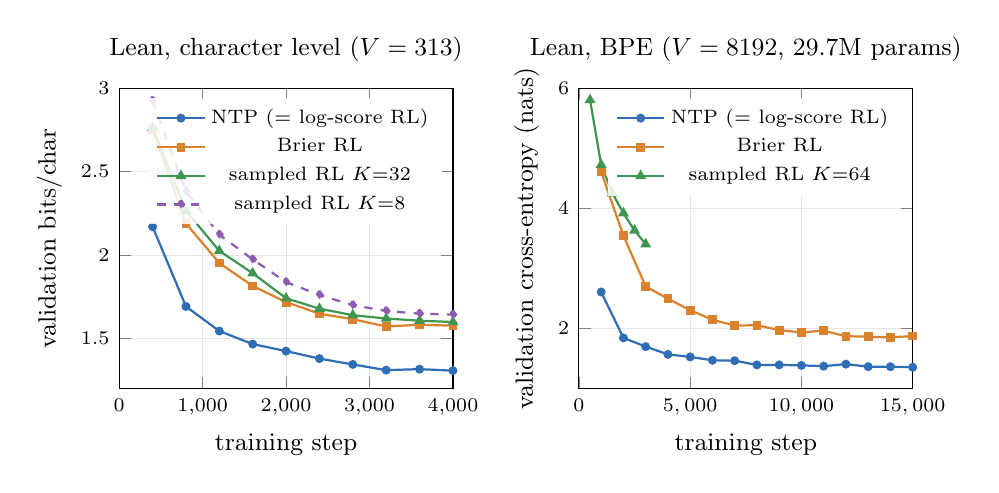
\begin{tikzpicture}
\begin{groupplot}[group style={group size=2 by 1,horizontal sep=1.6cm},
  width=0.48\linewidth,height=5.4cm,grid=major,grid style={black!10},
  tick label style={font=\scriptsize},label style={font=\small},title style={font=\small},
  legend style={font=\scriptsize,draw=none,fill=white,fill opacity=0.85,text opacity=1}]
\nextgroupplot[title={Lean, character level ($V=313$)},xlabel={training step},ylabel={validation bits/char},ymin=1.2,ymax=3.0,xmin=0,xmax=4000,legend pos=north east]
\addplot[ntp,thick,mark=*,mark size=1.2pt] coordinates {(400,2.171) (800,1.693) (1200,1.546) (1600,1.468) (2000,1.426) (2400,1.381) (2800,1.346) (3200,1.312) (3600,1.318) (4000,1.309)};
\addplot[brier,thick,mark=square*,mark size=1.2pt] coordinates {(400,2.753) (800,2.190) (1200,1.953) (1600,1.816) (2000,1.719) (2400,1.650) (2800,1.617) (3200,1.573) (3600,1.584) (4000,1.578)};
\addplot[pg,thick,mark=triangle*,mark size=1.5pt] coordinates {(400,2.764) (800,2.266) (1200,2.026) (1600,1.892) (2000,1.742) (2400,1.680) (2800,1.641) (3200,1.621) (3600,1.608) (4000,1.600)};
\addplot[pgb,thick,dashed,mark=diamond*,mark size=1.5pt] coordinates {(400,2.925) (800,2.382) (1200,2.123) (1600,1.975) (2000,1.839) (2400,1.762) (2800,1.701) (3200,1.666) (3600,1.650) (4000,1.645)};
\legend{NTP (= log-score RL),Brier RL,sampled RL $K{=}32$,sampled RL $K{=}8$}
\nextgroupplot[title={Lean, BPE ($V=8192$, 29.7M params)},xlabel={training step},ylabel={validation cross-entropy (nats)},ymin=1.0,ymax=6.0,xmin=0,xmax=15000,legend pos=north east,scaled x ticks=false,xticklabel style={/pgf/number format/1000 sep={,}}]
\addplot[ntp,thick,mark=*,mark size=1.2pt] coordinates {(1000,2.611) (2000,1.847) (3000,1.702) (4000,1.573) (5000,1.531) (6000,1.475) (7000,1.468) (8000,1.398) (9000,1.398) (10000,1.390) (11000,1.377) (12000,1.411) (13000,1.369) (14000,1.368) (15000,1.359)};
\addplot[brier,thick,mark=square*,mark size=1.2pt] coordinates {(1000,4.608) (2000,3.547) (3000,2.705) (4000,2.498) (5000,2.308) (6000,2.149) (7000,2.053) (8000,2.058) (9000,1.977) (10000,1.939) (11000,1.967) (12000,1.875) (13000,1.868) (14000,1.854) (15000,1.878)};
\addplot[pg,thick,mark=triangle*,mark size=1.5pt] coordinates {(500,5.804) (1000,4.727) (1500,4.255) (2000,3.921) (2500,3.634) (3000,3.406)};
\legend{NTP (= log-score RL),Brier RL,sampled RL $K{=}64$}
\end{groupplot}
\end{tikzpicture}
\caption{Validation loss of Transformers trained from rewards alone, compared with NTP. All curves descend; the RL curves lag by a roughly constant factor in steps that grows with the vocabulary.}\label{fig:curves}
\end{figure}

\paragraph{Result 2: the price is statistical, not computational.} Per training step, RL and NTP cost the same: the forward and backward passes dominate, and sampling $K$ tokens, counting collisions and computing $\|q\|^2$ are cheap (Table~\ref{tab:cost}). The difference lies in how much each step teaches. Table~\ref{tab:eff} reports, for each RL run, the number of steps NTP needed to reach the same quality (by interpolating the NTP curve), and the ratio.

\begin{table}[t]
\centering
\caption{Per-step cost relative to NTP (median of three interleaved rounds on a shared GPU; ratios are the meaningful quantity).}\label{tab:cost}
\small
\begin{tabular}{lccc}
\toprule
Scale & Method & Time per step & Peak memory \\
\midrule
\multirow{3}{*}{Character level, $V=313$} & \textsf{brier} & 0.93$\times$ & 1.04$\times$ \\
 & \textsf{pg} $K=8$ / $32$ & 0.95$\times$ / 0.94$\times$ & 1.04$\times$ / 1.05$\times$ \\
 & \textsf{pg} $K=128$ & 1.11$\times$ & 1.66$\times$ \\
\midrule
\multirow{2}{*}{BPE, $V=8192$} & \textsf{brier} & 1.15$\times$ & 1.12$\times$ \\
 & \textsf{pg} $K=8$ / $64$ & 1.13$\times$ / 1.21$\times$ & 1.44$\times$ / 1.44$\times$ \\
\bottomrule
\end{tabular}
\end{table}

\begin{table}[t]
\centering
\caption{Statistical efficiency: steps an RL run took, steps NTP needed to reach the same value, and their ratio.}\label{tab:eff}
\small
\begin{tabular}{lllrrr}
\toprule
Setting & Metric & Method & RL steps & NTP-equivalent & Ratio \\
\midrule
\multirow{4}{*}{Synthetic, $V=16$} & \multirow{3}{*}{$\KL(\mu\|q)$} & \textsf{brier} & 4000 & 1077 & 3.7 \\
 & & \textsf{pg8} & 4000 & 870 & 4.6 \\
 & & \textsf{pg2} & 4000 & 549 & 7.3 \\
 & $\|q-\mu\|^2$ & \textsf{brier} / \textsf{pg8} & 4000 & 3196 / 2932 & 1.3 / 1.4 \\
\midrule
\multirow{3}{*}{Lean char, $V=313$} & \multirow{3}{*}{bits/char} & \textsf{brier} & 4000 & 1126 & 3.6 \\
 & & \textsf{pg32} & 4000 & 1052 & 3.8 \\
 & & \textsf{pg8} & 4000 & 931 & 4.3 \\
\midrule
\multirow{2}{*}{Lean BPE, $V=8192$} & \multirow{2}{*}{cross-entropy} & \textsf{brier} & 15000 & 2117 & 7.1 \\
 & & \textsf{pg64} & 3000 & 578 & 5.2 \\
\bottomrule
\end{tabular}
\end{table}

\paragraph{Result 3: the gap is mostly the scoring rule, as Proposition~\ref{prop:poly} predicts.} The ratios decompose. Comparing \textsf{brier} with NTP isolates the choice of scoring rule (Brier versus logarithmic) with no sampling at all: $3.6$--$3.7\times$ at small vocabularies and $7.1\times$ at $V=8192$. Comparing \textsf{pg}$K$ with \textsf{brier} isolates sampling noise: an extra $1.05$--$1.25\times$ for $V\le313$, decreasing with $K$, and $1.4\times$ at $V=8192$ with $K=64$ (Brier reaches the cross-entropy that \textsf{pg64} attains at step $3000$ after about $2130$ steps). The scoring-rule term grows with the vocabulary for a simple reason: the logit gradient of the log score on the correct token is $1-q(x)$, whereas that of the Brier score is $q(x)(1-2q(x)+\|q\|^2)\approx q(x)$, which vanishes when $q(x)$ is small, and early in training $q(x)\approx1/V$. At BPE scale this is decisive: at every step the NTP model scores higher than the Brier-trained model \emph{even on the Brier score} ($0.284$ versus $0.273$ at step $15{,}000$). The metric also matters: on squared error, the Brier rule's own divergence, Brier-RL needs only $1.3\times$ the NTP steps on the synthetic source. Since sampled-token learners are confined to polynomial, Brier-type objectives (Proposition~\ref{prop:poly}), they inherit this price.

\begin{thesis}[What Experiment I shows]
RL from scalar rewards does learn next-token prediction in a real Transformer, at the same cost per step. The efficient instance of this RL is the one that takes the expectation over actions analytically with the logarithmic score, which is NTP itself. Any RL-native design should therefore keep this instance as its data reward and spend sampling only where no analytic expectation exists.
\end{thesis}

% ==================================================================
\section{Experiment II: Rewards That NTP Cannot Use}\label{sec:exp2}
% ==================================================================

\begin{plain}[The question]
If NTP is the dense, analytic corner of RL, what does the rest of RL buy? The clearest case is a reward that has no corpus behind it: a proof checker. NTP can only imitate proofs that already exist; RL can learn from the checker alone. Can a small model that has never seen a proof of the target problems learn to produce them, and what goes wrong?
\end{plain}

\paragraph{Setup.} Each experiment starts from a model pretrained on Lean code (Section~\ref{sec:exp1}). For each statement the model samples tactic proofs; Lean checks them; the reward is $1$ if Lean accepts the proof and $0$ otherwise, with group-normalized advantages. Optionally the stage-1 proper reward on corpus text is kept as an \emph{anchor} with weight $\lambda$, so that the objective is a single mixture of a data reward and a verifier reward. No proof examples are ever shown.

\paragraph{Toy propositions.} With the character-level model, randomly generated core-Lean goals from 12 templates (introduction and elimination of $\wedge,\vee,\to$, simple arithmetic) and one-line proofs, pass@1 on 48 held-out goals rose from $1.3\%$ to $22.9\%$ with the verifier reward alone, and to $52.1\%$ with the fair-Brier anchor ($\lambda=0.5$). Without the anchor the policy collapsed onto a single answer (\texttt{simp}) within 50 steps and stayed there; with it, the model learned to cite the relevant hypothesis (\texttt{simp [h2]}), producing nine distinct correct proof forms. This is Section~\ref{sec:tokens} in action: a pure 0--1 task reward is mode-seeking, and a proper data reward preserves the diversity that further learning needs.

\paragraph{miniF2F, one line.} With the BPE model we used the Lean~4 statements of miniF2F~\cite{zheng2022minif2f} distributed with DeepSeek-Prover-V1.5~\cite{xin2024deepseekprover15}; $423$ of $488$ elaborate under our Mathlib version. RL runs on the \texttt{valid} split and evaluation on the $212$ \texttt{test} problems. The reference point is a strong automation baseline: trying each of ten tactics (\texttt{grind}, \texttt{nlinarith}, \texttt{omega}, \texttt{linarith}, \texttt{ring\_nf}, \texttt{aesop}, \texttt{norm\_num}, \texttt{decide}, \texttt{simp}, \texttt{positivity}) solves $89$ test problems. Before RL the model solves $23$ (16 samples per problem). After 60 RL steps it solves $76$--$80$ with the verifier reward and the anchor; adding larger groups and a diversity reward lifts this to $84$ on both seeds (Table~\ref{tab:minif2f}). Across all runs RL solves $88$ problems, three of them beyond the baseline through tactic combinations such as \texttt{ring <;> norm\_num <;> grind}.

\paragraph{Reward hacking appears exactly where the reward is not proper.} Our diversity bonus first rewarded textually distinct correct proofs; the policy learned to pad \texttt{grind} with irrelevant lemma hints (\texttt{grind [add\_assoc]}, \texttt{grind [mul\_comm]}). Rewarding distinct tactic sequences instead, it learned to repeat tactics (\texttt{grind <;> grind <;> grind}). Both are instances of reward hacking~\cite{skalse2022hacking}: a diversity measure defined on the surface form can be satisfied by changing the surface form. A strictly proper data reward is immune to this particular failure, because its expectation is maximized only by the true distribution, whatever the surface; this is a practical argument for proper scores as the diversity-preserving term.

\paragraph{miniF2F, multi-line, with goal states.} Finally we let the model write proofs step by step. After each step Lean reports the remaining goals, which are shown to the model as a comment; best-first search orders partial proofs by cumulative log-probability and discards steps that do not change the goal. RL is expert iteration~\cite{anthony2017exit,polu2023curriculum}: search on the \texttt{valid} split, reward every step of every accepted proof, raise its probability under the anchor, repeat twice. Table~\ref{tab:minif2f} and Fig.~\ref{fig:minif2f} report the results. The search with automation tactics as additional candidates solves $94$ problems, above the $89$ baseline. The honest reading, however, is that the credit belongs to the search: a search over the same ten tactics with no model at all also solves $94$, at similar cost, and all five problems beyond the baseline are two-tactic combinations such as \texttt{aesop} followed by \texttt{nlinarith}. What RL demonstrably buys is efficiency: searching with the RL-trained policy alone solves $86$ problems with $3.7$ Lean calls per problem on average, against $20$ before RL; the ten-tactic baseline needs $10$ calls for $89$ and the tactic-only search $20.3$ calls for $94$. With automation candidates added, RL halves the verifier calls ($47.0\to21.6$) and the wall-clock time ($24\to9$ minutes) at the same solve rate.

\begin{table}[t]
\centering
\caption{miniF2F test ($212$ problems), Lean~4 and Mathlib. ``Beyond'' counts problems the ten-tactic baseline does not solve; ``calls'' is the mean number of Lean checks per problem. One-line rows: mean over two seeds, 60 RL steps, 16 samples per problem at evaluation.}\label{tab:minif2f}
\small
\begin{tabular}{lrrr}
\toprule
Method & Solved & Beyond & Calls \\
\midrule
Ten automation tactics, each tried once (baseline) & 89 & -- & 10 \\
Tactic-only best-first search, no model & 94 & 5 & 20.3 \\
\midrule
\multicolumn{4}{l}{\emph{One-line proofs, sampled}} \\
\quad pretrained model, no RL & 23 & 0 & 16 \\
\quad RL: verifier reward + anchor $\lambda=0.5$ & 78 & 0 & 16 \\
\quad RL: + larger groups, stronger anchor, diversity reward & 84 & 0.5 & 16 \\
\midrule
\multicolumn{4}{l}{\emph{Multi-line proofs, best-first search with goal states}} \\
\quad pretrained model, policy only & 20 & 0 & 14.9 \\
\quad RL (expert iteration), policy only & 86 & 2 & \textbf{3.7} \\
\quad pretrained model + automation candidates & 93 & 5 & 47.0 \\
\quad RL + automation candidates & 94 & 5 & 21.6 \\
\bottomrule
\end{tabular}
\end{table}

\begin{figure}[t]
\centering
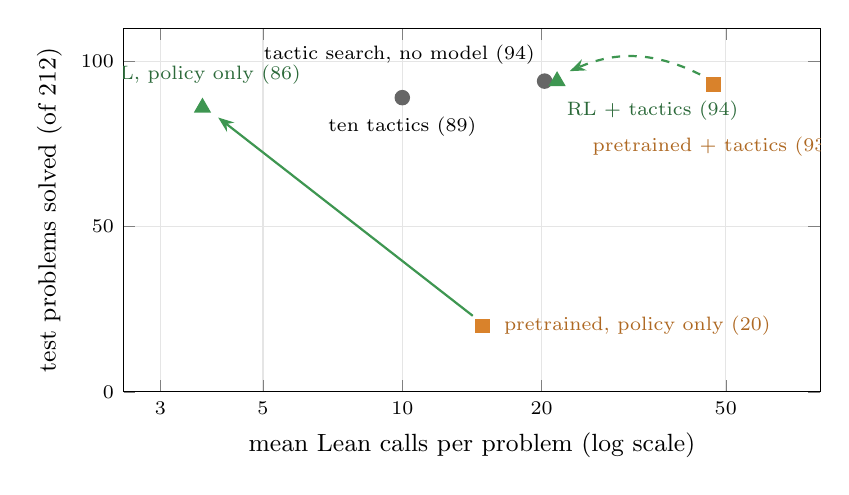
\begin{tikzpicture}
\begin{axis}[width=0.86\linewidth,height=6.2cm,xlabel={mean Lean calls per problem (log scale)},ylabel={test problems solved (of 212)},
  xmode=log,xmin=2.5,xmax=80,ymin=0,ymax=110,grid=major,grid style={black!10},
  xtick={3,5,10,20,50},xticklabels={3,5,10,20,50},
  tick label style={font=\scriptsize},label style={font=\small}]
\draw[-{Stealth[length=2mm]},pg,thick] (axis cs:14.2,23) -- (axis cs:4.0,83);
\draw[-{Stealth[length=2mm]},pg,thick,dashed] (axis cs:44,96) to[bend right=25] (axis cs:23,97);
\addplot[only marks,mark=*,mark size=2.6pt,color=black!60] coordinates {(10,89) (20.3,94)};
\addplot[only marks,mark=square*,mark size=2.4pt,color=brier] coordinates {(14.9,20) (47.0,93)};
\addplot[only marks,mark=triangle*,mark size=3.2pt,color=pg] coordinates {(3.7,86) (21.6,94)};
\node[font=\scriptsize,anchor=north] at (axis cs:10,86) {ten tactics (89)};
\node[font=\scriptsize,anchor=south east] at (axis cs:20.3,96) {tactic search, no model (94)};
\node[font=\scriptsize,anchor=north west,pg!70!black] at (axis cs:21.6,91) {RL + tactics (94)};
\node[font=\scriptsize,anchor=north,brier!80!black] at (axis cs:47,80) {pretrained + tactics (93)};
\node[font=\scriptsize,anchor=west,brier!80!black] at (axis cs:15.8,20) {pretrained, policy only (20)};
\node[font=\scriptsize,anchor=south,pg!70!black] at (axis cs:3.7,90) {RL, policy only (86)};
\end{axis}
\end{tikzpicture}
\caption{Solve rate against verifier cost on miniF2F test. Arrows show the effect of RL from the verifier. RL turns a model that cannot prove into one that reaches $97\%$ of the automation baseline at a third of its cost, but at this scale it does not exceed what search over automation already achieves.}\label{fig:minif2f}
\end{figure}

\paragraph{Two pitfalls worth reporting.} Both changed our numbers substantially and are easy to repeat. First, batching many candidate proofs into one Lean file lets a malformed candidate (for example, a lone comment after \texttt{by}) push its parse error onto the next theorem, so that it is scored as correct; error attribution must account for this, and comments and search commands such as \texttt{exact?} must be rejected. Second, byte-level BPE merges the newline after \texttt{by} with the following indentation, so a prompt that ends in a bare newline is out of distribution: our model then produced comments and new declarations, and assigned probability zero to \texttt{grind}. Ending the prompt at \texttt{by} fixed this.

\begin{thesis}[What Experiment II shows]
A verifier is a reward NTP cannot use, and RL from it turns a model that has never seen a proof into a competent, cheap prover, with no demonstrations. Pure task rewards collapse the policy; a proper data reward in the same objective counteracts collapse and, unlike surface-level diversity bonuses, cannot be gamed by rewriting. At $30$M parameters the learned policy reproduces, and makes far cheaper, the competence latent in its pretraining and in Lean's automation; exceeding that competence requires capacity this study did not have.
\end{thesis}

% ==================================================================
\section{Toward RL-Native Language Models: A Research Program}\label{sec:program}
% ==================================================================

The usual pipeline treats a language model as a predictor first and an agent second. The results above suggest treating it as an agent throughout, with prediction as the agent's densest reward. We call this the RL-native view and state it as one objective.

\paragraph{One objective.} For a policy $\pi_\theta$ over token sequences, a data distribution $\mathcal D$, a strictly proper scoring rule $S$ and task rewards $r_j$ with environments $\mathcal E_j$,
\begin{equation}\label{eq:unified}
J(\theta)\;=\;\lambda\,\underbrace{\E_{x\sim\mathcal D}\sum_t S\big(\pi_\theta(\cdot\mid x_{<t}),x_t\big)}_{\text{data reward: analytic, dense, proper}}\;+\;\sum_j\beta_j\,\underbrace{\E_{e\sim\mathcal E_j,\;y\sim\pi_\theta(\cdot\mid e)}\,r_j(e,y)}_{\text{task rewards: sampled, sparse}} .
\end{equation}
With $S=S_L$ and $\beta_j=0$ this is pretraining. With $\lambda=0$ it is RL with verifiable rewards and its collapse. Everything in between is a single reward-maximization problem, with one schedule for $\lambda$ and $\beta_j$ in place of a hand-off between stages. Section~\ref{sec:tokens} explains why the data term should stay ($\lambda>0$): it is the only term in~\eqref{eq:unified} whose optimum is a distribution rather than a mode, and Experiment~II shows that it is the term that cannot be gamed by surface rewriting. Fig.~\ref{fig:pipeline} contrasts the two views.

\begin{figure}[t]
\centering
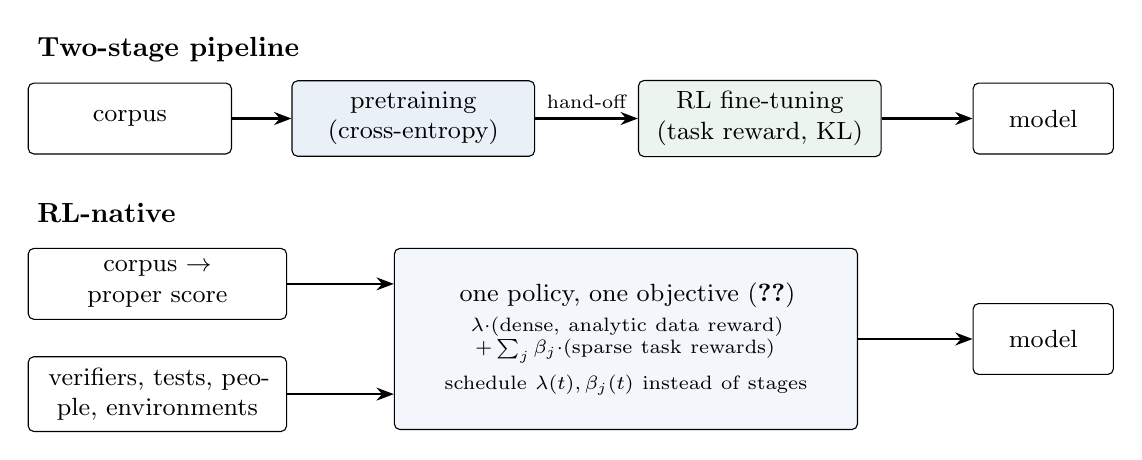
\begin{tikzpicture}[font=\small,
  box/.style={draw,rounded corners=2pt,align=center,minimum height=0.9cm,inner sep=4pt,fill=white},
  arr/.style={-{Stealth[length=2.2mm]},thick}]
% row 1: two-stage pipeline
\node[font=\bfseries,anchor=south west] at (-1.3,0.6) {Two-stage pipeline};
\node[box,text width=2.3cm] (c1) at (0,0) {corpus};
\node[box,text width=2.8cm,fill=ntp!10] (p1) at (3.6,0) {pretraining\\(cross-entropy)};
\node[box,text width=2.8cm,fill=pg!10] (r1) at (8.0,0) {RL fine-tuning\\(task reward, KL)};
\node[box,text width=1.5cm] (m1) at (11.6,0) {model};
\draw[arr] (c1) -- (p1); \draw[arr] (p1) -- node[above,font=\scriptsize]{hand-off} (r1); \draw[arr] (r1) -- (m1);
% row 2: RL-native
\node[font=\bfseries,anchor=south west] at (-1.3,-1.45) {RL-native};
\node[box,text width=3.0cm] (c2) at (0.35,-2.1) {corpus $\to$ proper score};
\node[box,text width=3.0cm] (v2) at (0.35,-3.5) {verifiers, tests, people, environments};
\node[box,text width=5.6cm,fill=boxbg,minimum height=2.3cm] (j2) at (6.3,-2.8) {one policy, one objective~\eqref{eq:unified}\\[3pt]\scriptsize$\lambda\cdot$(dense, analytic data reward)\\\scriptsize$+\sum_j\beta_j\cdot$(sparse task rewards)\\[2pt]\scriptsize schedule $\lambda(t),\beta_j(t)$ instead of stages};
\node[box,text width=1.5cm] (m2) at (11.6,-2.8) {model};
\draw[arr] (c2.east) -- (j2.west|-c2.east); \draw[arr] (v2.east) -- (j2.west|-v2.east); \draw[arr] (j2) -- (m2);
\end{tikzpicture}
\caption{The two-stage pipeline and the RL-native view. In the latter, pretraining is not a separate paradigm but the densest, analytically computable reward in a single objective.}\label{fig:pipeline}
\end{figure}

\paragraph{What has to be solved.} The program is only as good as its open problems. We list those our analysis and experiments expose, in rough order of urgency.
\begin{enumerate}[leftmargin=*,label=\textbf{P\arabic*.},itemsep=3pt]
\item \textbf{Keep the analytic corner.} Wherever an expectation over actions can be computed in closed form, as it can for next-token rewards on data, compute it, and use the log score. Experiment~I shows that giving this up costs $3.6$--$7.1\times$ in steps. Sampling should be reserved for rewards that only exist as black boxes.
\item \textbf{Variance and vocabulary.} Sampled-token learning degrades as the vocabulary grows, because the chance that a sample hits the observed token is small. Control variates that exploit the known structure of~\eqref{eq:unified}, importance sampling from a proposal concentrated near the data token, and hierarchical or factorized action spaces are natural directions, as is a theory of how many samples per context a fair group reward needs as a function of the entropy of $\mu_t$.
\item \textbf{Proper rewards at the level of responses.} Our token-level results lift directly only to rewards on whole responses when those rewards are themselves proper scores of a distribution. Designing sequence-level fair rewards that are cheap to estimate from a group of sampled responses, and whose optimum is a calibrated distribution over correct answers rather than one answer, is the response-level analogue of Proposition~\ref{prop:two}.
\item \textbf{Semantic, not syntactic, diversity.} Experiment~II shows that diversity defined on surface forms is gamed immediately. Diversity measured on meaning (for proofs: proof terms or goal trajectories; for programs: behavior on tests) is needed wherever a proper data reward is unavailable.
\item \textbf{Verifiable environments as the new corpus.} If pretraining is the data reward, then curated environments with checkable rewards, such as formal mathematics, program synthesis and simulators, play the role that text corpora play today. Their scale, diversity and curricula become first-class research objects~\cite{polu2023curriculum,yang2023leandojo}.
\item \textbf{Exploration and irreversibility.} All guarantees above live in non-reactive environments. In interactive settings with irreversible actions no policy matches the informed optimum (Section~\ref{sec:limits}); RL-native models that act in the world need weaker, history-relative optimality notions and safe exploration.
\item \textbf{Scaling laws for the mixture.} How should $\lambda$ and $\beta_j$ evolve with compute? Our data suggest that early training should be dominated by the analytic data reward, which is most informative per step, and that sparse rewards pay off once the prior places non-negligible probability on rewarded behavior, as the jump from $20$ to $86$ problems illustrates.
\end{enumerate}

% ==================================================================
\section{Where the Slogan Stops}\label{sec:limits}
% ==================================================================

``All you need'' is a claim about sufficiency in principle. It is important to say exactly where it holds.

\begin{proposition}[No universal policy against informed optimal policies]\label{prop:trap}
Let $E_L,E_R$ be two computable environments that look identical before the first action; in $E_L$ choosing left leads to an absorbing state with reward $1$ forever and right to one with reward $0$; $E_R$ is the mirror image. A policy choosing left with probability $\theta$ earns average reward $\theta$ in $E_L$ and $1-\theta$ in $E_R$, while the informed optimal policy earns $1$ in both; in one of them the regret grows at least as $T/2$.
\end{proposition}

\noindent The obstruction is informational and holds for incomputable policies too~\cite{lattimore2011asymptotic,leike2015bad}. Prediction environments escape it because a wrong prediction costs reward but never information. Table~\ref{tab:notions} summarizes what is and is not established.

\begin{table}[t]
\centering
\caption{Readings of ``reinforcement learning is all you need'' and their status.}\label{tab:notions}
\small
\begin{tabular}{>{\raggedright}p{7.6cm}>{\raggedright\arraybackslash}p{6.8cm}}
\toprule
Reading & Status \\
\midrule
RL can express every probabilistic prediction task, NTP included & True with a strictly proper reward (Lemma~\ref{lem:regret}, Corollary~\ref{cor:ntp}) \\
One policy has bounded regret on all computable prediction environments & True, incomputable policy (Theorems~\ref{thm:universal}, \ref{thm:token}) \\
Same, with single-sample token rewards & False (Proposition~\ref{prop:single}, Theorem~\ref{thm:quadratic}) \\
Ordinary policy gradient learns NTP from rewards alone & Observed at small scale, $3.6$--$7.1\times$ slower in steps (Section~\ref{sec:exp1}) \\
RL from a verifier learns skills without demonstrations & Observed at small scale; did not exceed automation plus search (Section~\ref{sec:exp2}) \\
One policy is near-optimal in all computable interactive environments & False against informed benchmarks (Proposition~\ref{prop:trap}); weaker notions partly true~\cite{lattimore2011asymptotic,leike2016thompson} \\
RL-native training beats the two-stage pipeline at scale & Open; this paper proposes, it does not show \\
\bottomrule
\end{tabular}
\end{table}

\paragraph{Further caveats.} The universal policy is incomputable; the universality theorems say nothing about which policy a practical algorithm finds. Our experiments use models of $5$--$30$M parameters, one GPU and mostly one seed; effects at frontier scale may differ in either direction. The miniF2F results compare favorably with a strong automation baseline only in cost, not in solve rate. Finally, Corollary~\ref{cor:ntp} cuts both ways: it shows that NTP is RL, and it also shows that, for data rewards, the best RL algorithm is NTP. The RL-native view gains its content from what it adds to NTP, not from replacing it.

% ==================================================================
\section{Conclusion}\label{sec:conclusion}
% ==================================================================

Next-token prediction and reinforcement learning are not two paradigms. With a strictly proper scoring rule as reward, the first is the special case of the second in which the environment ignores the agent and the expectation over actions can be taken exactly; the familiar cross-entropy loss is the policy gradient of the logarithmic score. Through this identity the RL framework inherits Solomonoff's universality on prediction tasks, and with a fair two-sample reward it does so even in the token-sampling format that language models use. Ordinary Transformers trained from scalar rewards alone do learn to predict, at the cost per step of NTP and with a statistical price that the theory traces to the scoring rule. And the same framework holds the rewards that imitation cannot use: a proof checker alone taught a small model, shown no proofs, to prove competition problems cheaply, with a proper data reward guarding it against collapse.

In this precise sense, reinforcement learning is all you need: one reward-maximization objective can specify the whole training of a language model, with pretraining as its densest reward. Whether models trained that way will one day surpass the two-stage pipeline is an empirical question that this paper raises rather than settles. The program of Section~\ref{sec:program} is our proposal for how to find out.

\paragraph{Code and data.} Lean sources, training and evaluation scripts, and all result files are available from the author on request and will accompany the preprint.

% ==================================================================
\appendix
\section{Proofs}\label{app:proofs}
% ==================================================================

\paragraph{Theorem~\ref{thm:hutter}.} Dominance gives $\ln(\mu^{(n)}/\xi^{(n)})\le\ln(1/c)$ pointwise on the support of $\mu^{(n)}$, hence $\KL(\mu^{(n)}\|\xi^{(n)})\le\ln(1/c)$. The chain rule gives $\KL(\mu^{(n)}\|\xi^{(n)})=\sum_{t\le n}\E_\mu\KL(\mu_t\|\xi_t)$. For $p,q\in\Del$, $\|p-q\|_2^2\le\frac12\|p-q\|_1^2\le\KL(p\|q)$ by Pinsker's inequality~\cite{csiszar1967}. The partial sums of $\|\xi_t-\mu_t\|^2$ are non-decreasing with bounded expectations, so the infinite sum is finite almost surely and its terms tend to zero.

\paragraph{Theorem~\ref{thm:quadratic}.} Let $g(z)$ be the gradient of $\Omega$ at interior $z$ along $T_0$. Since interior $p$ maximizes the differentiable $J_p$, its directional derivatives vanish: $\langle Rp+g(p),v\rangle=0$ for $v\in T_0$, i.e.\ $\langle g(z),v\rangle=-v^\top Rz$ for all interior $z$. For interior $p,q$ and $d=q-p$, $\varphi(s)=\Omega(p+sd)$ has $\varphi'(s)=-d^\top R(p+sd)$, so $\Omega(q)-\Omega(p)=-d^\top Rp-\frac12d^\top Rd$. Since $U_\rho(q;p)-U_\rho(p;p)=d^\top Rp$, adding gives $J_p(q)-J_p(p)=-\frac12d^\top Rd$; continuity extends this to $q\in\Del$. For $\Omega=\beta H$ the second derivative along $e_a-e_b$ is $-\beta(1/q(a)+1/q(b))$, which is not constant, so entropy (and KL, which differs by a linear term) is excluded; and a quadratic divergence is never $\KL(p\|q)$.

\paragraph{Proposition~\ref{prop:vstat}.} $\E\sum_{k,l}\one\{A_k=A_l\}=K+K(K-1)\|q\|^2$ gives the expression for $U$. Completing the square, $U=-c\|q-p/c\|^2+\mathrm{const}$, so the maximizer is the projection, which has the thresholding form with $\tau>0$ because $\sum_ap(a)/c=1/c>1$. Subtracting $\tau>0$ from $p(a)/c>p(b)/c>\tau$ strictly increases their ratio, and coordinates with $p(a)/c\le\tau$ are clipped to zero.

\paragraph{Proposition~\ref{prop:poly}.} $U_\rho(q;p)=\sum_{a_{1:K},x}q(a_1)\cdots q(a_K)\,p(x)\,\rho(a_{1:K},x)$ is a polynomial, bounded on the compact set $\Del\times\Del$, whereas $\KL(p\|q)\to\infty$ as $q(a)\to0$ with $p(a)>0$.

% ==================================================================
\section{Experimental Details}\label{app:exp}
% ==================================================================

\paragraph{Models and optimization.} Decoder-only Transformers with learned positional embeddings and pre-layer normalization. Character-level runs: AdamW, learning rate $10^{-3}$ with $100$ warm-up steps and cosine decay, batch $64\times128$ (Lean) or $64\times64$ (synthetic), dropout $0.1$ on text. BPE runs: width $512$, $8$ layers, $8$ heads, context $512$, tied embeddings, AdamW ($\beta=(0.9,0.95)$, weight decay $0.1$), learning rate $6\times10^{-4}$ with $500$ warm-up steps and cosine decay to $10\%$, batch $32\times512$, bfloat16 autocast. Sampled-token rewards use per-sample credit $r_k=2\one\{A_k=x\}-w\,\#\{l\ne k:A_l=A_k\}$ with $w=2/(K-1)$ (fair) or $2/K$ (biased) and a batch-mean baseline.

\paragraph{Verifier RL.} Toy propositions: core Lean without Mathlib, one file per candidate, 8 goals $\times$ 8 samples per step, 200 steps, learning rate $10^{-4}$. miniF2F one-line: 8 problems $\times$ 16 or 32 samples per step, 60 steps, learning rate $2\times10^{-5}$, anchor on 8 corpus windows per step; diversity reward shares a unit reward among identical correct proofs in a group and adds a one-time novelty bonus of $0.5$. Multi-line: best-first search with 8 policy samples per expansion, at most 6 expansions and depth 6; steps that leave the goal unchanged or revisit a state are pruned; expert iteration uses two rounds of search on \texttt{valid} with at most 4 expansions, three epochs over the accepted steps, anchor $\lambda=0.5$. Lean checks batch 16 candidates per file under \texttt{import Mathlib} with \texttt{maxHeartbeats 400000}; candidates containing comments, \texttt{sorry}, \texttt{admit}, \texttt{native\_decide}, search commands or declaration keywords are rejected before checking, and a nine-case regression test guards error attribution.

\paragraph{Hardware and software.} One NVIDIA RTX PRO 4000 Blackwell laptop GPU (16\,GB), 20 CPU cores, PyTorch~2.13, Lean~4.34.1 with Mathlib v4.34.1 for verification and Lean~4.35.0 for core-Lean checks.

\bibliographystyle{unsrt}
\bibliography{refs}

\end{document}
